\documentclass{beamer}

\usetheme{Madrid}
\usecolortheme{default}

\title{Metodi del Calcolo Scientifico}
\subtitle{Progetto 2}
\author{Francesco~Refolli.~865955}
%\logo{\includegraphics[height=1cm]{logo_unimib.pdf}}

\newcommand{\putimagecouple}[4] {
  \begin{figure}[!htb]
      \centering
      \begin{minipage}{0.45\linewidth}
          \centering
          \includegraphics[width=\linewidth]{#1}
          \caption{#2}
      \end{minipage}
      \hspace{0.25cm}
      \begin{minipage}{0.45\linewidth}
          \centering
          \includegraphics[width=\linewidth]{#3}
          \caption{#4}
      \end{minipage}
  \end{figure}
}

\begin{document}

\frame{\titlepage}

\begin{frame}
\frametitle{Indice}
\tableofcontents
\end{frame}

\section{Introduzione}

\begin{frame}
\frametitle{Introduzione}

Implementazione delle operazioni:
\begin{itemize}
  \item DCT-II
  \item DCT-II 2D
  \item IDCT-II
  \item IDCT-II 2D
\end{itemize}

e dell'algoritmo di compressione simil-jpeg

\begin{figure}
  \centering
  \includegraphics[height=1cm]{images/cpp.png}
  \hspace{0.5cm}
  \includegraphics[height=1cm]{images/eigen.png}
  \hspace{0.5cm}
  \includegraphics[height=1cm]{images/fftw.png}
  \hspace{0.5cm}
  \includegraphics[height=1cm]{images/pocketfft.png}
\end{figure}

\end{frame}

\section{Libreria}

\begin{frame}
\frametitle{Architettura}
\begin{figure}
  \centering
  \includegraphics[width=\linewidth]{images/diagram.png}
\end{figure}
\end{frame}

\begin{frame}
\frametitle{Algoritmo di Compressione}
\begin{figure}
  \centering
  \includegraphics[width=\linewidth]{images/ad-compression.png}
\end{figure}
\end{frame}

\subsection{Interfacce}

\begin{frame}
\frametitle{Interfacce - CLI}
\begin{figure}
  \centering
  \includegraphics[width=\linewidth]{images/interface-cli.png}
\end{figure}
\end{frame}

\begin{frame}
\frametitle{Interfacce - GUI}
\begin{figure}
  \centering
  \includegraphics[width=\linewidth]{images/interface-gui.png}
\end{figure}
\end{frame}

\section{Esperimenti}

\begin{frame}
\frametitle{Benchmark DCT - Confronto Generale}
\begin{figure}
  \centering
  \includegraphics[width=0.67\linewidth]{images/actuator-trends.png}
\end{figure}
\end{frame}

\begin{frame}
\frametitle{Benchmark DCT - Focus sulle Librerie}
\putimagecouple{images/benchmark-libraries-wsl.png}{WSL}{images/benchmark-libraries-linux.png}{Linux}
\end{frame}

\begin{frame}
\frametitle{Benchmark Compressione}
\putimagecouple{images/benchmark-compression-wsl.png}{WSL}{images/benchmark-compression-linux.png}{Linux}
\end{frame}

\begin{frame}
\frametitle{Compressione di Immagini - Grayscale - Originale}
\begin{figure}
  \centering
  \includegraphics[width=\linewidth]{images/compression-gs-original.png}
\end{figure}
\end{frame}

\begin{frame}
\frametitle{Compressione di Immagini - Grayscale - F=30/d=10}
\begin{figure}
  \centering
  \includegraphics[width=\linewidth]{images/compression-gs-F30-d10.png}
\end{figure}
\end{frame}

\begin{frame}
\frametitle{Compressione di Immagini - Dimensione dei Blocchi - Originale}
\begin{figure}
  \centering
  \includegraphics[width=0.58\linewidth]{images/compression-gb-original.png}
\end{figure}
\end{frame}

\begin{frame}
\frametitle{Compressione di Immagini - Dimensione dei Blocchi - F=8/d=2}
\begin{figure}
  \centering
  \includegraphics[width=0.58\linewidth]{images/compression-gb-F8-d2.png}
\end{figure}
\end{frame}

\begin{frame}
\frametitle{Compressione di Immagini - Dimensione dei Blocchi - F=128/d=30}
\begin{figure}
  \centering
  \includegraphics[width=0.58\linewidth]{images/compression-gb-F128-d30.png}
\end{figure}
\end{frame}

\begin{frame}
\frametitle{Compressione di Immagini - Colori - Originale}
\begin{figure}
  \centering
  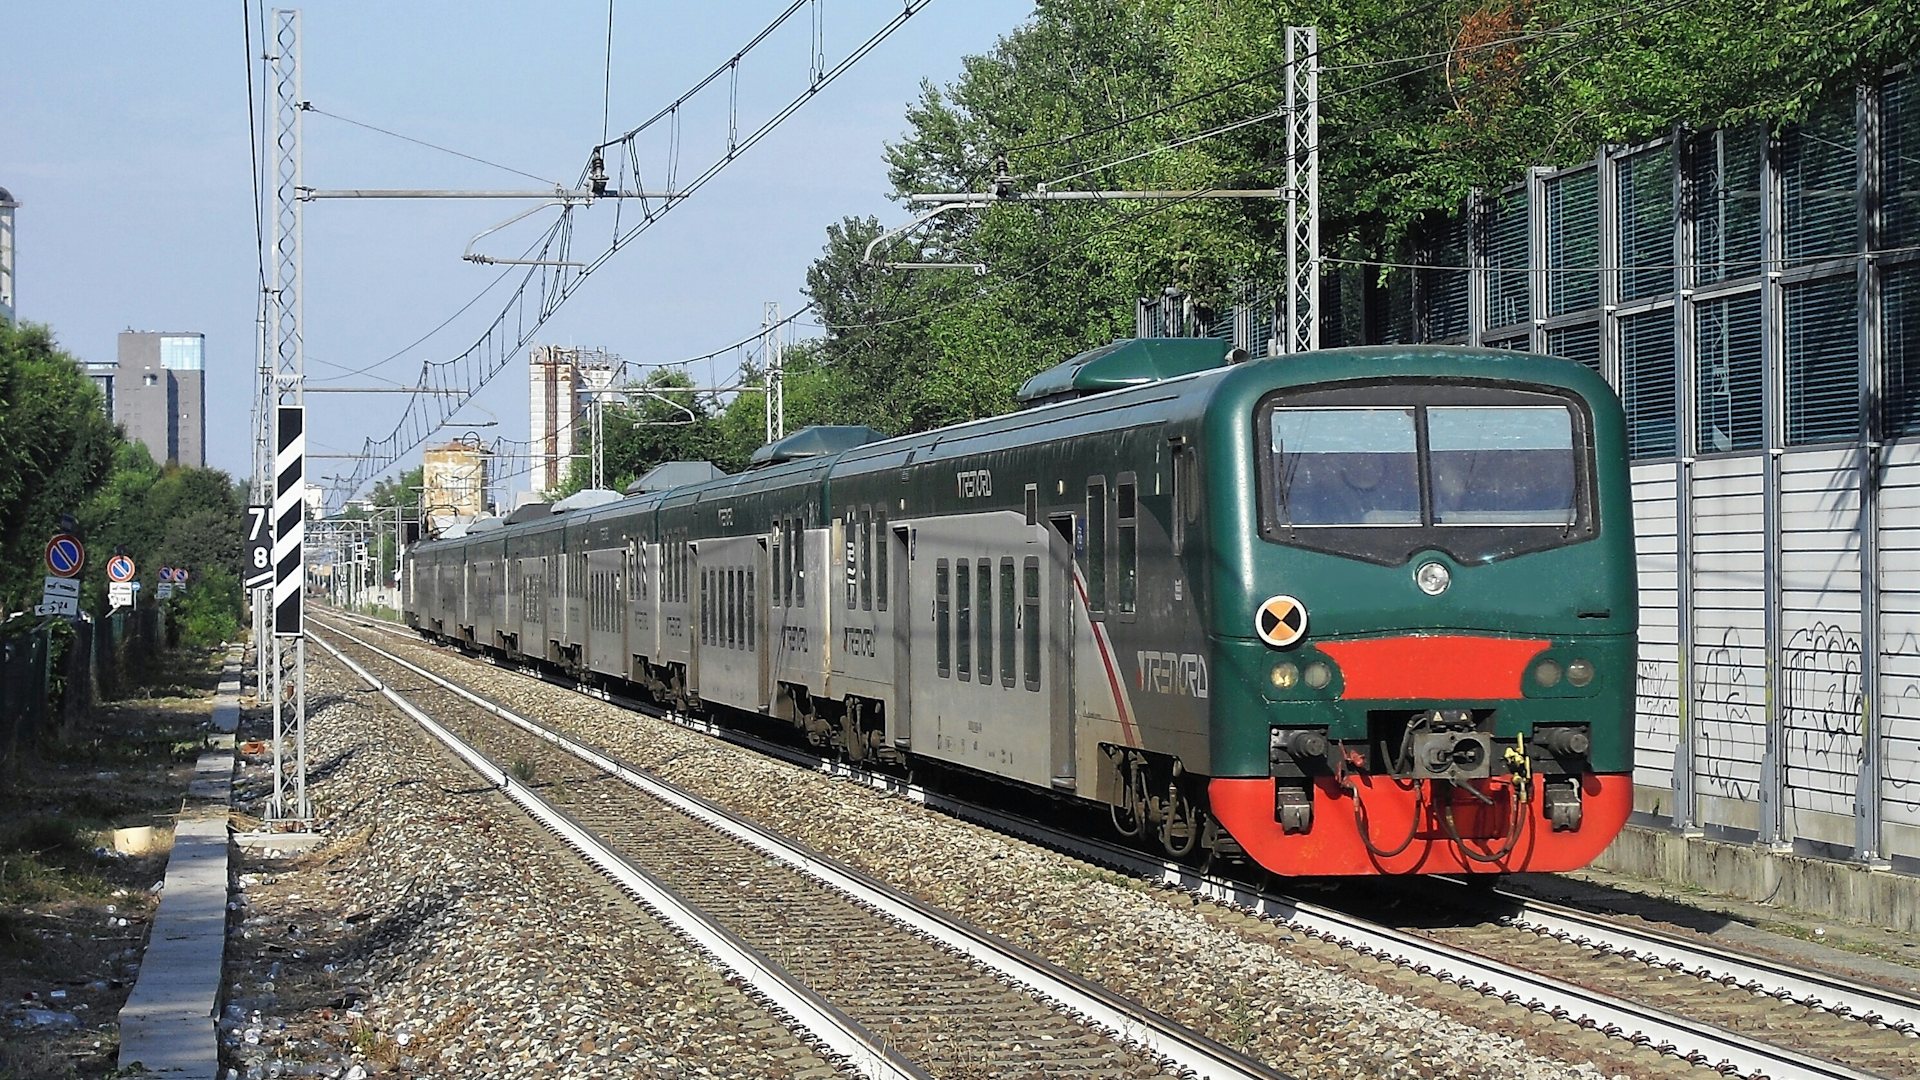
\includegraphics[width=\linewidth]{images/compression-cl-original.png}
\end{figure}
\end{frame}

\begin{frame}
\frametitle{Compressione di Immagini - Colori - F=30/d=10}
\begin{figure}
  \centering
  \includegraphics[width=\linewidth]{images/compression-cl-F30-d10.png}
\end{figure}
\end{frame}

\begin{frame}
\centering
\Huge
Fine
\end{frame}

\end{document}
